\placelogofalse
\begin{frame}{Introduction}
\begin{columns}
\column{0.58\linewidth}
\centering
\begin{outline}
  \1 LBM is a framework for numerically modeling Fluid dynamics
  \1 Historically, not great for turbulence
  \1 New collision operators like CM-MRT improve this
  \1 Adoption for graphics research \cite{Li2020, Li2024, Lyu2021}
\end{outline}

\column{0.38\linewidth}
\begin{center}
\centering
\shadowimage[width=2.5cm]{li2020_image.png}

\shadowimage[width=2.5cm]{lyu2021_image.png} 
\end{center}
\end{columns}
\end{frame}
\placelogotrue

\placelogofalse
\begin{frame}{Results}
  \begin{center}
  \centering
  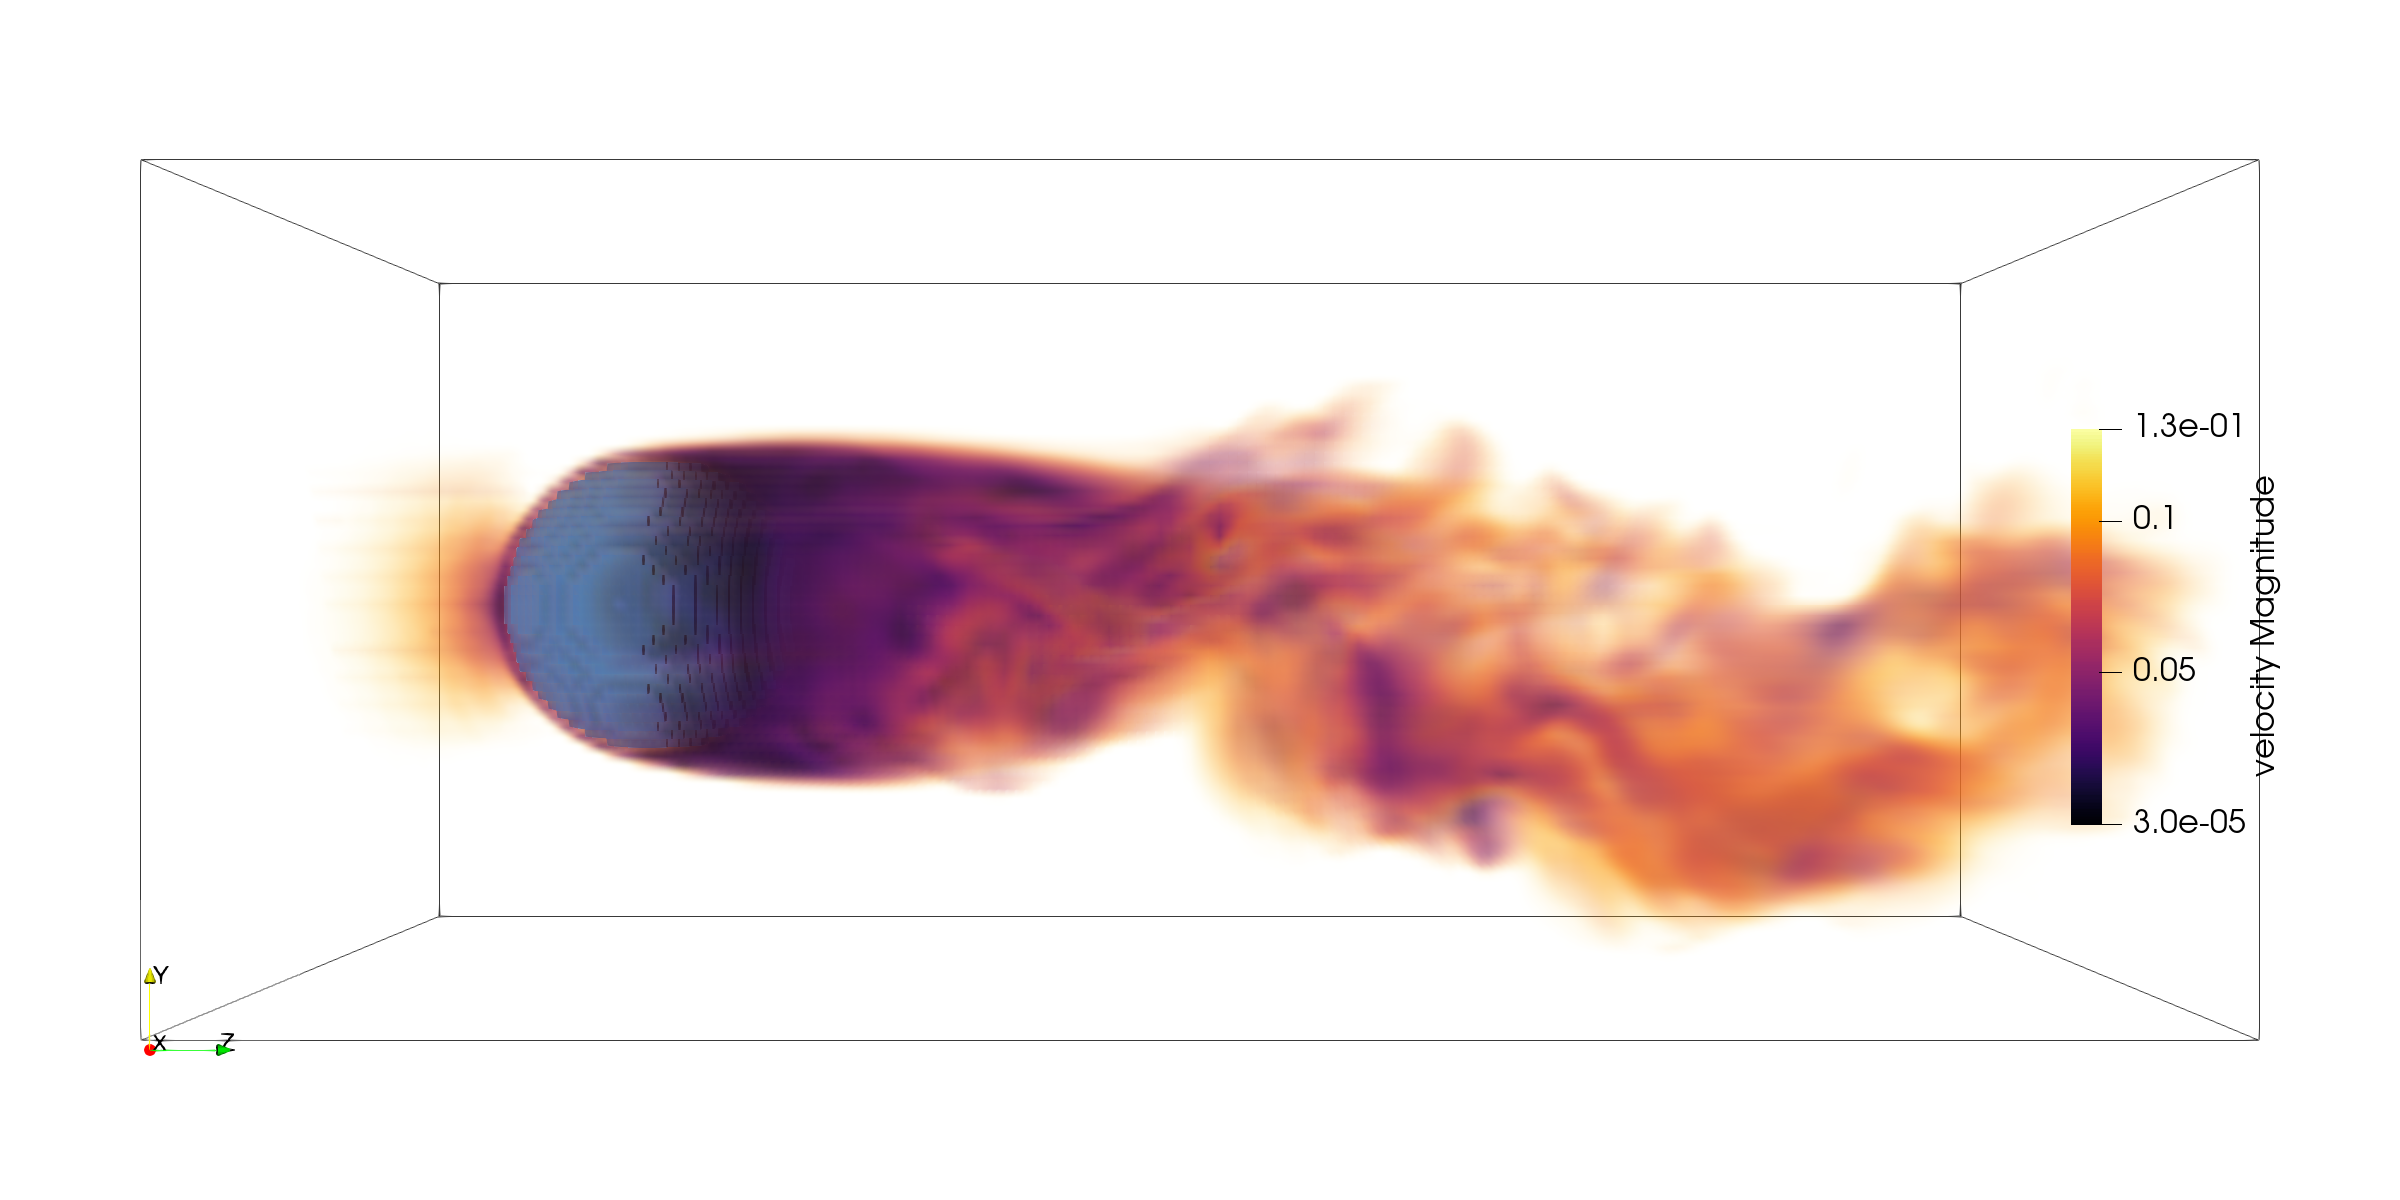
\includegraphics[width=\linewidth]{purple_render.png}
  \end{center}
\end{frame}
\placelogotrue
